\section{Numerical Experiments}

\subsection{Monochromatic Filters}
Monochromatic approximation can work well only if color components span few one dimensional subspaces. 
Figures \ref{AlexNetComponents}, \ref{MattNetComponents} show that it is indeed case for both AlexNet, as
well as MattNet. In case of AlexNet, we colored with a different colors every feature map, so one dimensional structure
is clearly depicted. For MattNet, we found further low-dimensional structure. All the colors seems to lay close
to two planes. Visualization gives different color to color components laying on every plane. Moreover,
colors span one dimensional subspaces within planes.

\begin{figure}[t]
\mbox{
  \subfigure[AlexNet]{
      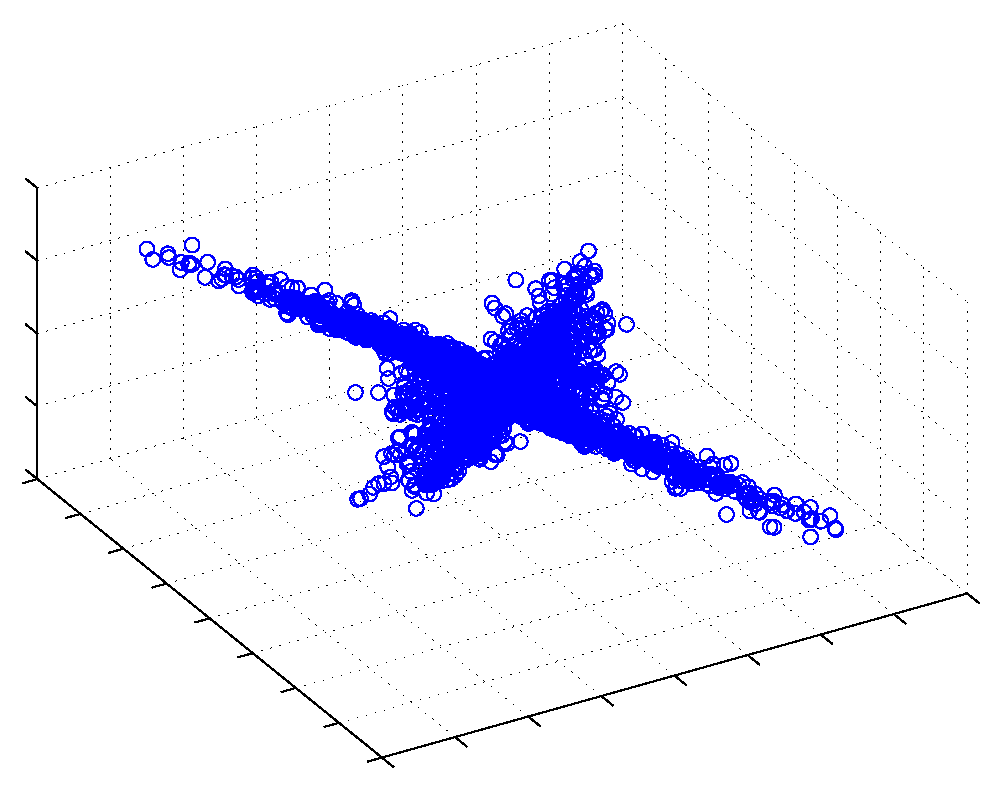
\includegraphics[width=0.48\linewidth]{img/color_components_alex_3d.eps}
      \label{AlexNetComponents}
  }\quad
\subfigure[MattNet]{
  \includegraphics[width=0.48\linewidth]{img/color_components_matthew_3d.eps} 
  \label{MattNetComponents}
  }
}
\caption{Visualization of color components for AlexNet and MattNet.}
\end{figure}



\subsection{Biclustering}

